\documentclass[tikz,border=2mm]{standalone}
\usepackage{pgfplots}
\pgfplotsset{compat=1.18}

\begin{document}
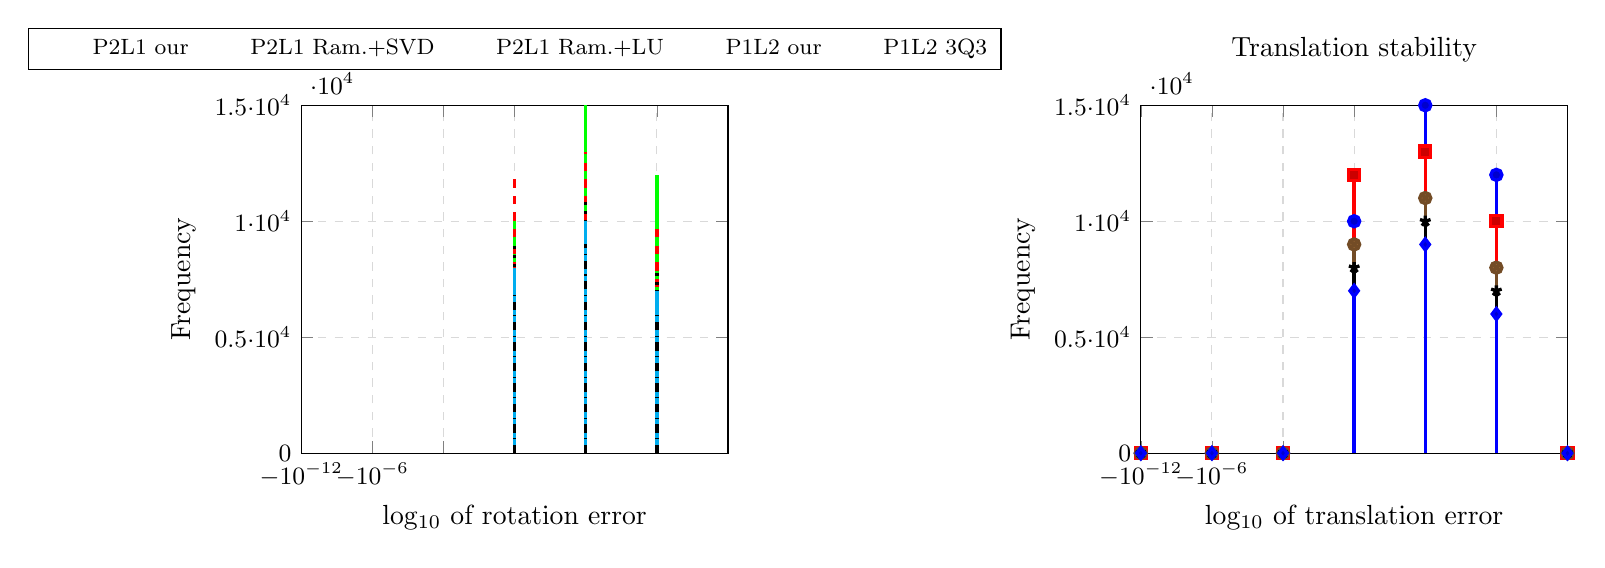
\begin{tikzpicture}
    \begin{axis}[
        name=ax1,
        width=7cm, height=6cm,
        xlabel={log$_{10}$ of rotation error},
        ylabel={Frequency},
        xmin=-18, xmax=-6,
        ymin=0, ymax=1.5e4,
        xticklabels={$-10^{18}$,$-10^{-12}$,$-10^{-6}$},
        ytick={0,0.5e4,1e4,1.5e4},
        yticklabels={0,0.5$\cdot 10^4$,1$\cdot 10^4$,1.5$\cdot 10^4$},
        grid=major,
        grid style={dashed, gray!30},
        ticklabel style={font=\small},
        legend style={at={(0.5,1.1)}, anchor=south,legend columns=-1,font=\footnotesize},
        cycle list={
            {green,solid},
            {red,dashed},
            {black,dotted},
            {cyan,solid},
            {black,dashdotted}
        },
        title={Rotation stability},
        title style={align=center, at={(0.5,1.05)}}
    ]
        % Data points for histograms
        \addplot+ [ycomb, very thick] coordinates {
            (-18, 0) (-16, 0) (-14, 0) (-12, 10000) (-10, 15000) (-8, 12000) (-6, 0)
        };
        \addplot+ [ycomb, very thick] coordinates {
            (-18, 0) (-16, 0) (-14, 0) (-12, 12000) (-10, 13000) (-8, 10000) (-6, 0)
        };
        \addplot+ [ycomb, very thick] coordinates {
            (-18, 0) (-16, 0) (-14, 0) (-12, 9000) (-10, 11000) (-8, 8000) (-6, 0)
        };
        \addplot+ [ycomb, very thick] coordinates {
            (-18, 0) (-16, 0) (-14, 0) (-12, 8000) (-10, 10000) (-8, 7000) (-6, 0)
        };
        \addplot+ [ycomb, very thick] coordinates {
            (-18, 0) (-16, 0) (-14, 0) (-12, 7000) (-10, 9000) (-8, 6000) (-6, 0)
        };

        \legend{P2L1 our, P2L1 Ram.+SVD, P2L1 Ram.+LU, P1L2 our, P1L2 3Q3}
    \end{axis}

    \begin{axis}[
        at={(ax1.right of south east)},
        anchor=left of south west,
        width=7cm, height=6cm,
        xlabel={log$_{10}$ of translation error},
        ylabel={Frequency},
        xmin=-18, xmax=-6,
        ymin=0, ymax=1.5e4,
        xticklabels={$-10^{18}$,$-10^{-12}$,$-10^{-6}$},
        ytick={0,0.5e4,1e4,1.5e4},
        yticklabels={0,0.5$\cdot 10^4$,1$\cdot 10^4$,1.5$\cdot 10^4$},
        grid=major,
        grid style={dashed, gray!30},
        ticklabel style={font=\small},
        title={Translation stability},
        title style={align=center, at={(0.5,1.05)}}
    ]
        % Data points for histograms
        \addplot+ [ycomb, very thick] coordinates {
            (-18, 0) (-16, 0) (-14, 0) (-12, 10000) (-10, 15000) (-8, 12000) (-6, 0)
        };
        \addplot+ [ycomb, very thick] coordinates {
            (-18, 0) (-16, 0) (-14, 0) (-12, 12000) (-10, 13000) (-8, 10000) (-6, 0)
        };
        \addplot+ [ycomb, very thick] coordinates {
            (-18, 0) (-16, 0) (-14, 0) (-12, 9000) (-10, 11000) (-8, 8000) (-6, 0)
        };
        \addplot+ [ycomb, very thick] coordinates {
            (-18, 0) (-16, 0) (-14, 0) (-12, 8000) (-10, 10000) (-8, 7000) (-6, 0)
        };
        \addplot+ [ycomb, very thick] coordinates {
            (-18, 0) (-16, 0) (-14, 0) (-12, 7000) (-10, 9000) (-8, 6000) (-6, 0)
        };
    \end{axis}
\end{tikzpicture}
\end{document}